\section{Background and Problem Formulation}
\label{sec:background}
In this section, we review the three categories of systems from Table~\ref{tab:intro-landscape}.
For each category, we describe how it specializes query execution and where it falls short.
We then formalize workload-specialized query rewriting.

\subsection{Rule-based Rewriting in DBMSs}
\label{sec:bg_rules}
Rule-based rewriting frameworks~\cite{PiraheshHH92} express transformations as rules over the logical plan.
Each rule has a structural pattern and a transformation.
The optimizer applies rules repeatedly until a fixpoint (no rule fires anymore) or a budget is reached.
Extensible frameworks, such as Apache Calcite~\cite{Calcite} \blue{and Orca~\cite{Orca}}, apply rules in a fixed sequence or through cost-based search.
These systems are efficient and deterministic, but their coverage is limited.
Missing transformation opportunities that no rule encodes are invisible to the optimizer.
For example, the \texttt{COUNT(*)} star-join factorization is a form of eager aggregation~\cite{YanL95,ChaudhuriS94} and factorized joins~\cite{BakibayevKOZ13}.
It speeds up some Stats-CEB queries by orders of magnitude, yet PostgreSQL~18 and MySQL do not implement it.
PostgreSQL~19 adds eager aggregation~\cite{PG19}, three decades after the technique was published.
\blue{Subquery decorrelation shows the same gap: it has been expressed as composable rewrite rules for decades~\cite{GalindoLegaria01}, yet general unnesting of complex queries is still being improved~\cite{UnnestingBTW25}.}

\textbf{Limitations:} Rule discovery systems extend the rule set automatically.
WeTune~\cite{WeTune} enumerates and verifies rewrite rules over a relational algebra template space.
QueryBooster~\cite{QueryBooster} generalizes rules from user-provided examples.
GRewriter~\cite{GRewriter} mines rewrite patterns from query logs to expand the rule set of the optimizer.
LearnedRewrite~\cite{learnedrewrite} uses Monte Carlo Tree Search over existing Calcite rules to find better rule orders.
\blue{Steered optimizers, such as QO-Advisor~\cite{SteeringQO, QOAdvisor}, learn rule configurations offline from recurring production jobs and deploy them as deterministic hints, but they only enable or disable rules the optimizer already has.}
\blue{AutoSteer~\cite{AutoSteer} learns per query which optimizer rules and knobs to disable on engines such as PostgreSQL and DuckDB, and likewise stays within the existing rule set.}
These systems reduce manual rule engineering.
However, each one works within a bounded space: a template grammar, user examples, logged patterns, or an existing rule set.
A rewrite outside this space remains out of reach.
\blue{SlabCity~\cite{SlabCity} reaches such rewrites through program synthesis instead of rules, but it searches per query and leaves no reusable rule behind.}
So the host optimizer, with or without these extensions, is not specialized to the transformations a given workload needs.

\vspace{-0.15cm}
\subsection{LLM-based Query Rewriting}
\label{sec:bg_llm}
LLMs can find rewrites for concrete queries, beyond predefined rule spaces.
R-Bot~\cite{RBot} and LLM-R2~\cite{LLMR2} use the LLM to select and order existing Calcite rules, improving how a rule set is used, but cannot add missing transformations.
GenRewrite~\cite{GenRewrite} and ReSequel~\cite{resequel} rewrite whole queries.
GenRewrite accumulates natural-language rewrite rules and passes them as hints to the LLM for later queries.
It still calls the LLM per query. \blue{LITHE~\cite{LITHE} also rewrites each query with the LLM, combining an ensemble of prompts with a Monte Carlo Tree Search guided by the LLM's token probabilities. LLM-QO~\cite{LLMQO} goes further and fine-tunes an LLM to generate execution plans directly.} The recent ReSequel outperforms R-Bot, LLM-R2, and LearnedRewrite~\cite{resequel}.
It masks constants to group queries into templates, and prompts the LLM with each template, catalog metadata, and example rules, and the LLM returns several rewritten variants. ReSequel checks the variants on downsampled data and selects the fastest one.
A template cache stores the verified variants, so later queries of the same template reuse them without LLM calls.
Queries of unseen templates go to an offline layer, which calls the LLM asynchronously or on demand.

\textbf{Limitations:} ReSequel faces three limitations.
First, its LLM costs grow with the number of templates.
On TPC-H, DSB, and Stats-CEB, every query forms its own template~\cite{resequel}.
Template reuse pays off only on workloads with heavy repetition, such as IMDB, where 13,646 queries map to 79 templates.
Second, a template matches only queries with the same structure and schema.
A new query that shares a fragment with a past query, but differs in number of tables, is a new template; causing a new LLM call.
Third, ReSequel selects rewrites on data samples, which can distort cardinalities.
On StackOverflow at scale factor 12, it slows down 53 PostgreSQL queries.
Across all these systems, the output is a rewritten query or template; nothing they learn persists as reusable knowledge.
\blue{Two recent systems turn LLM output into rules.}
\blue{QO-Verify~\cite{Narasayya26} verifies LLM rewrites with the transformation rules of the SQL Server optimizer; rewrites it cannot verify expose missing rules, which optimizer developers then derive by hand.}
\blue{Mallet~\cite{Mallet} generates rules with an LLM offline and reuses them without LLM calls, but for SQL dialect translation rather than query optimization.}

\vspace{-0.15cm}
\subsection{Workload-specific Engine Synthesis}
\label{sec:bg_synthesis}
Engine synthesis specializes the whole engine instead of the query.
BespokeOLAP~\cite{bespokeolap} takes a \emph{DBMS contract}, which consists of a set of SQL query templates and a Parquet dataset.
An LLM coding agent then generates a complete C++ engine for this contract.
The agent first plans the storage layout.
It then implements each query and optimizes the code in several rounds, guided by runtime profiles.
A validation loop compares results against DuckDB, and a hotpatching infrastructure keeps each iteration short.
The generated engines target in-memory execution.
On their target workloads, they outperform DuckDB by an order of magnitude or more~\cite{bespokeolap}.

\textbf{Limitations:} This specialization comes at a cost.
Synthesis costs \$276 in LLM tokens for the 22 TPC-H templates and \$303 for the 16 CEB templates, and takes 10--30 hours~\cite{bespokeolap}.
The engine is specialized only to its contract.
Queries outside the contract fall back to a general-purpose engine, such as DuckDB.
A lasting workload change requires re-synthesis.
The generated engine also replaces the host and its abstraction layers, so it must re-implement data loading, parallel execution, and memory management per workload.
It is read-only over a Parquet snapshot, so data changes require reloading and rebuilding~\cite{bespokeolap}.
In our experiments with CEB at scale factors 1 to 10, loading and preprocessing take 63\% to 73\% of every run.
In our runs, its query execution gains at most $1.69\times$ from 32 threads, while DuckDB gains $5.5\times$ to $7.8\times$ on the same queries after our rewrites.

\subsection{Problem Formulation}
\label{sec:problem}
Let $\mathcal{W}$ be an evolving workload over a database $\mathcal{D}$.
We observe a sample $\mathcal{Q}_s \subseteq \mathcal{W}$ and must serve future queries $\mathcal{W}'$, which include queries not in $\mathcal{W}$.
Let $\ell(Q)$ be the latency of query $Q$ on the host engine.
A rewrite produces $Q' \equiv Q$, and a useful rewrite should yield latency improvements $\ell(Q') < \ell(Q)$. In the following, we introduce key concepts and the overall optimization objective. 

\begin{definition}[Fragments]
A \emph{fragment} is a subtree of the logical plan $P(Q)$.
A \emph{fragment key} is a canonical fingerprint of a fragment that keeps operator types, join kinds, and tree shape, and drops constants, table names, and column names.
For example, Stats-CEB queries~88 and~122 share the key \texttt{AGG(JOIN[INNER])}.
$\mathcal{K}(Q)$ denotes the fragment keys of all subtrees of $P(Q)$.
\end{definition}

\begin{definition}[Transformation Rule]
\label{def:rule}
A rule $r = (\phi_r, \tau_r, \mathcal{K}_r)$ has an applicability condition $\phi_r$ over plan fragments, a transformation $\tau_r$, and the fragment keys $\mathcal{K}_r$ under which it can fire.
It returns $r(Q) = \tau_r(Q)$ if $\phi_r(Q)$ holds and $r(Q) = Q$ otherwise, with $r(Q) \equiv Q$ whenever $\phi_r(Q)$ holds.
$\phi_r$ and $\tau_r$ refer to operator patterns and roles, not to constants, table names, or a fixed join arity.
\end{definition}

\textbf{Rule Distillation and Matching:}
For a sampled query $Q$, an LLM rewriter returns a candidate $Q'' = \mathrm{Rewriter}(Q)$ intended to be equivalent to $Q$.
Distillation extracts a set of candidate rules $\mathcal{R}^* = \mathrm{Distill}(Q, Q'')$ from the difference between $P(Q)$ and $P(Q'')$.
The challenge is to generalize each $\phi_{r^*}$ beyond the source query, so the rule applies to queries with different characteristics.
At rewrite time, only the rules $\mathcal{R}(Q) = \{ r \in \mathcal{R} \mid \mathcal{K}_r \cap \mathcal{K}(Q) \neq \emptyset \}$ evaluate $\phi_r$.
So matching cost grows with the matching rules. %, not with the rule set.

\begin{definition}[Rule Verification]
\label{def:verification}
Let $\mathcal{D}_s$ be a set of downsampled databases and $\mathcal{Q}_r$ the sampled queries on which $r$ fires when rewritten with $\mathcal{R} \cup \{r\}$ and that return a non-empty result on $\mathcal{D}_s$.
The test $\mathrm{Test}(r)$ returns $\mathsf{valid}$ iff $\mathcal{Q}_r \neq \emptyset$ and $\mathrm{Rewrite}(Q, \mathcal{R} \cup \{r\})$ and $Q$ return the same result on every database in $\mathcal{D}_s$, for all $Q \in \mathcal{Q}_r$.
$\mathrm{Verify}(r, \mathcal{R}, \mathcal{Q}_s, \mathcal{D}_s)$ rejects $r$ if $\mathrm{Smoke}(r)$ fails or $\mathrm{SMT}(r) = \mathsf{NEQ}$, accepts $r$ if $\mathrm{SMT}(r) = \mathsf{EQ}$, and returns $\mathrm{Test}(r)$ if $\mathrm{SMT}(r)$ is $\mathsf{UNKNOWN}$ or $\mathsf{ERROR}$ (all described below).
A rule set $\mathcal{R}$ is \emph{verified} if $\mathrm{Verify}$ accepts every rule in it.
\end{definition}

\textbf{Rule Verification Costs:} The three verification alternatives have increasing cost.
The \emph{smoke test} $\mathrm{Smoke}(r)$ compiles $r$ and exercises $\phi_r$ on crafted micro-queries, which rejects code that fails to build or load.
The \emph{formal check} $\mathrm{SMT}(r)$ passes a sampled query $Q$ on which $r$ fires and its rewrite $r(Q)$ to a Satisfiability Modulo Theories (SMT) solver~\cite{SQLSolver}\blue{, following SMT-based equivalence provers such as EQUITAS~\cite{EQUITAS},} with time budget $B_{\mathit{smt}}$.
It returns $\mathsf{EQ}$, $\mathsf{NEQ}$ with a counterexample, $\mathsf{UNKNOWN}$, or $\mathsf{ERROR}$.
The \emph{result-equivalence test} $\mathrm{Test}(r)$ handles the cases the solver cannot decide.
Unlike the formal check, it rewrites with $\mathcal{R} \cup \{r\}$, so it also covers rule interactions.
To keep the cost low, it evaluates one query of $\mathcal{Q}_r$ per distinct firing sequence (Section~\ref{sec:offline:verify}).
Rules accepted by the formal check are proven equivalent, while rules accepted by the test agree empirically with the original queries on $\mathcal{D}_s$.


\begin{figure*}[t]
\vspace{-0.25cm}
    \resizebox{.95\textwidth}{!}{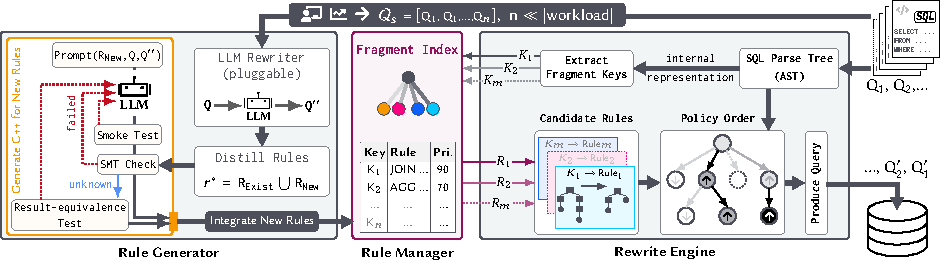
\includegraphics[scale=0.75]{figures/img/fig_ROLEX_Architecture}}
    \vspace{-0.35cm}
    \caption{{\sys} architecture: the offline \textbf{Rule Generator} (right) distills and verifies rules from a pluggable rewriter; the \textbf{Fragment Index} (middle) maps fragment keys to rules; the online \textbf{Rewrite Engine} (left) applies them in priority order to produce $Q'$.\shorten}
    \label{fig:system_arch}
    \vspace{-0.35cm}
\end{figure*}

\textbf{Optimization Objective:}
Given $\mathcal{D}$, a host engine, and a sample $\mathcal{Q}_s$, construct a rule set $\mathcal{R}$ and a rule ordering $\omega$ that minimize the execution time of future queries:
\begin{equation}
\min_{\mathcal{R},\,\omega} \sum_{Q \in \mathcal{W}'} \ell\!\left(\mathrm{Rewrite}(Q, \mathcal{R}, \omega)\right),
\end{equation}
subject to four constraints (in terms of requirements).
\begin{itemize}
\item \emph{(R1) Verified:} $\mathcal{R}$ is a verified rule set (see Definition~\ref{def:verification}).
\item \emph{(R2) LLM-free online:} online $\mathrm{Rewrite}$ uses only $\mathcal{R}$ and $\omega$.
\item \emph{(R3) Reusable:} $\phi_r$ and $\tau_r$ are independent of constants, tables, and join arity, so $r$ fires on unseen queries in $\mathcal{W}'$.
\item \emph{(R4) Non-invasive:} $\mathrm{Rewrite}$ maps SQL to SQL, and the host engine is not modified.
\end{itemize}
The LLM cost of building $\mathcal{R}$ is paid offline, once for the sample $\mathcal{Q}_s$, so it does not grow with the number of future queries or templates.
A query with no matching rule runs unchanged.
In Table~\ref{tab:intro-landscape}, the host optimizer meets R2 and R4 but is not specialized, ReSequel needs an LLM call for every new template and violates R3, and BespokeOLAP violates R3 and R4 and pays its cost per workload.